\section{Evaluation}
\label{sec:eval}

We would like to know, does multi-dispatch linearizability offer applications significantly lower end-to-end latency for realistic workloads compared to baselines (single-dispatch linearizability)?
The evaluation aims to answer this overarching question by answering following questions:

\begin{itemize}
\item How does the e2e application latency scale with the number of clients and the request fanout?

\item How does the number of shards impact the e2e app. latency of MDL?

\item What is the e2e app. latency of MDL in the wide area? How sensitive is it to configurations with diverse intershard distances?
\end{itemize}

\subsection{Experimental Set-up}
We implement a MDL key-value store that uses MDL-Paxos per shard, and the multi-dispatch protocol for cross-shard coordination.
\begin{itemize}
    \item Using 5(3) replicas per shard
    \item Using 5(2) shards
    \item Cloudlab, replicas and shards within single data center, 10Gbs local network
    \item Each server is 10 cores, Intel Xeon Silver 4114, 2.2GHz
\end{itemize}
The variables we vary:
\begin{itemize}
    \item Skew (uniform vs. zipfian)
    \item Number of clients
    \item Types of requests - RW, WO, RO
    \item Fan-out
    \item Number of keys
    \item Number of shards
    \item Request arrival-time
    \item Inter-shard distance
    \item Network lossiness?
        \subitem This would highlight the overhead of buffering that happens with out of order packets for MD-lin, but it might not be interesting if the metric is e2e app-req latency
    \item Failure rate
\end{itemize}

Metrics we measure:
\begin{itemize}
    \item e2e app. latency
    \item system level tput
\end{itemize}

To keep the load on the system the same between sdl and mdl, we increase the number of concurrent clients for sdl but keep it constant for mdl as the number of requests per client increases, keeping the overall number of requests sent to the system the same for both.

We also compare against different request types: read-only, write-only, and read-write. We expect to see a difference in performance for these since multiple read-only requests issued will never have conflicts, whereas the other two types can induce conflicts that lead to reissuing.

\subsection{MDL Microbenchmarks}

\begin{figure*}[hbt!]
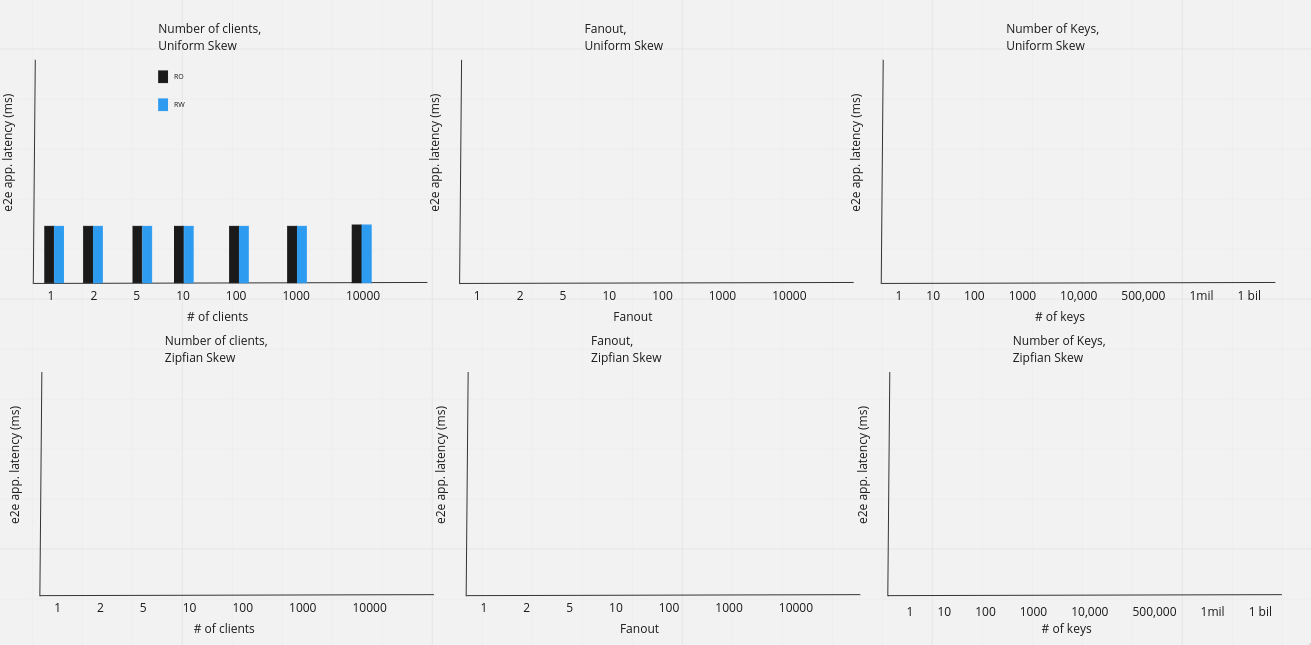
\includegraphics[scale=.36]{microbenchmarks.png}
\caption{Microbenchmarks.}
\label{fig:microben}
\end{figure*}

We are particularly interested in seeing how load and contention impact the performance of the MDL protocol. 
\begin{enumerate}
    \item With \textbf{increased load}, we expect bursty behavior, since the dependency propagation in the log will be across more entries.
    \item With \textbf{increased contention}, we expect significant slow downs of multi-dispatch due to the reissuing of requests.
\end{enumerate}  

The contention is most sensitive to
\begin{itemize}
    \item the number of clients
    \item the fanout
    \item the skew
    \item the number of keys
    \item type of request
\end{itemize}

We show 6 subplots in figure \ref{fig:microben}, where we vary each of these variables to see the fine grained impact.

We expect to see:
\begin{enumerate}
    \item num of clients: an increase in latency. since the logs will be longer, we have to propagate more dependencies
    \item fanout: an increase in latency, same as \# of clients.
    \item skew: an increase in latency, we expect to see more conflicts and thus more reissuing
    \item num of key: should see decrease in latency, less likely to have conflicts with more keys
    \item type of request: RO will have no reissuing, RW will have more reissing, so it will be slower
\end{enumerate}

Some todos:
\begin{itemize}
    \item TODO show plots for system-level throughput
    \item TODO should also probably vary zipfian
\end{itemize}

\subsection{Scaling Number of Shards}
In this section, we show how the MDL e2e application latency scales with the number of shards. 

As shown in figure \ref{fig:shard-scaling}, we expect app-level request latency will \textbf{scale reasonably well with an increased number of shards.} Assuming we hold the number of clients, fanout, skew/keyspace, and inter-shard RTT values constant, then the protocol shouldn't induce a significantly greater overhead with more shards. 
\begin{enumerate}
    \item In fact, since an increasing number of shards will likely balance the load at within each shard, \textbf{the per-shard processing and reordering will be faster, contributing to a speedup} (shorter logs). 
    \item The competing factor that will contribute to an increase in latency is the property that \textbf{conflicts will be more likely with an increased number of shards (more chance for reordering, since no single-shard sequence number ordering), so we will likely see more reissuing as we scale the number of shards.}
\end{enumerate}


\begin{figure}[!htb]
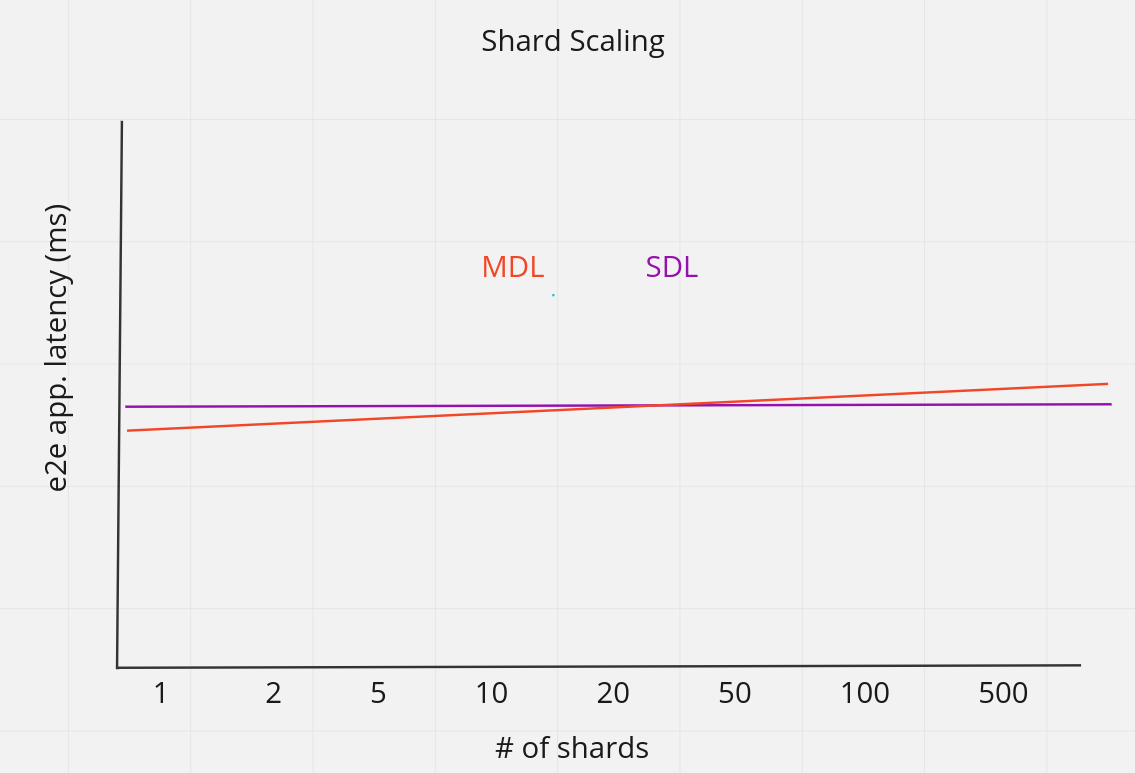
\includegraphics[scale=.20]{shard_scaling.png}
\caption{Multi-sharded MDL with increasing number of shards.}
\label{fig:shard-scaling}
\end{figure}

\subsection{MDL with Geo-rep in the Wide Area}
We show the e2e app. latency for varying inter-shard latency (which we call the wide area **this might be wrong terminology) and inter-replica latency (which we call geo-replication, also might be wrong terminology).

\begin{figure}[!htb]
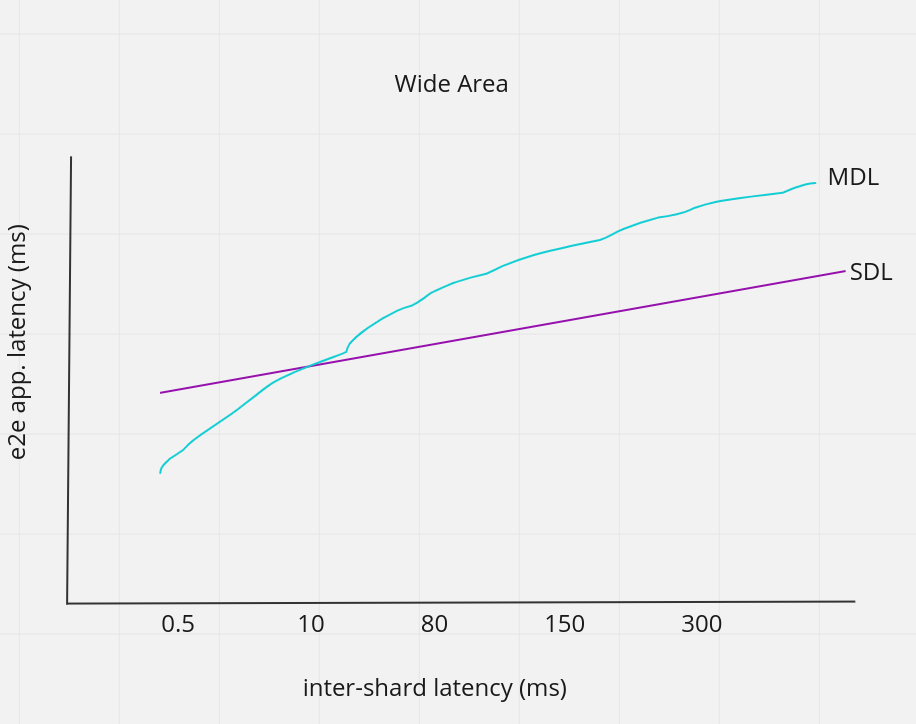
\includegraphics[scale=.24]{wide-area.png}
\caption{Multi-sharded MDL in the Wide Area}
\label{fig:wide-area}
\end{figure}
In figure \ref{fig:wide-area}, if we assume each shard is in a single data center (low inter-rep latency), with increasing inter-shard latency, \textbf{we expect the e2e app. latency for MDL to increase, since the inter-shard communication will take longer} which is fundamentally necessary for the protocol. We expect a small increase for SDL as well, since each subrequest will take a variable length of time, depending on which shard it must visit, but not a significant increase.

In figure \ref{fig:geo-rep}, if we assume a large inter-shard latency, as we increase the inter-replica latency, SDL latency will increase, but \textbf{we expect MDL latency to increase at a slower rate. This is because we can overlap} the inter-replica round trips that have to take place for committing log entries with the inter-shard round trips that have to take place to determine conflicts for log entries.
\begin{figure}[!htb]
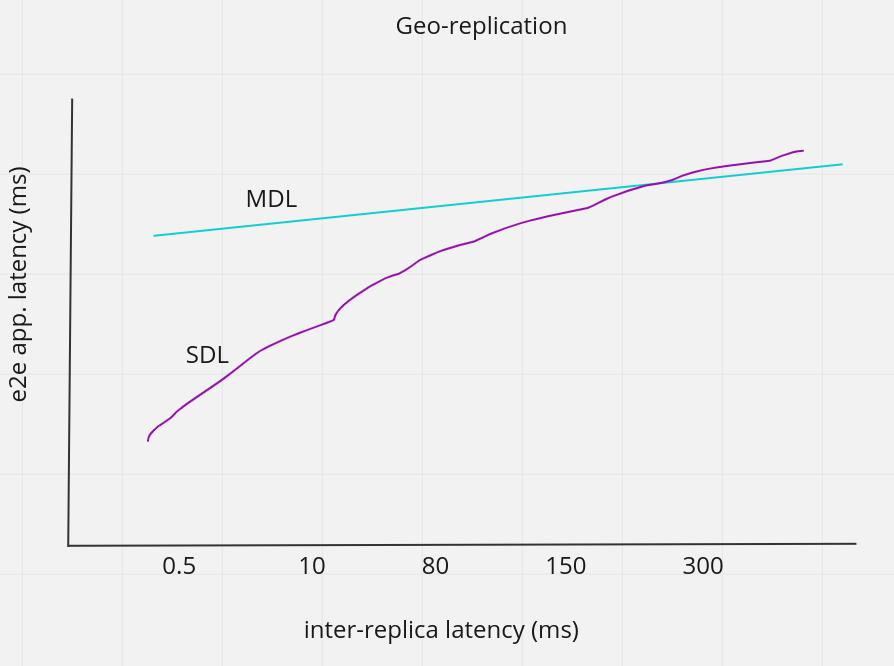
\includegraphics[scale=.25]{geo-rep.png}
\caption{Multi-sharded MDL with Geo-replication.}
\label{fig:geo-rep}
\end{figure}
